% Files using this must be two subfolders
% deep. Adjust the number of ../ for the
% depth of the file.
% Imports
\usepackage{fancyhdr}
\usepackage{geometry}
\usepackage{icomma}
\usepackage{amsmath}
\usepackage{multicol}
\usepackage{mathptmx}
\usepackage{anyfontsize}
\usepackage{t1enc}
\usepackage{tabto}
\usepackage{listings}
\usepackage{filecontents}
\usepackage{subcaption}
\usepackage{tikz}
\usepackage[parfill]{parskip}
\usepackage{graphicx}
\usepackage[]{mdframed}
\usepackage{amsmath}
\usepackage[makeroom]{cancel}
\usepackage{pgfplots}
\usepackage{pgfplotstable}
\usepackage{xfrac}
\usepackage{amssymb}
\usepackage{mathtools}
\pgfplotsset{compat=1.18}
\usetikzlibrary{patterns}
\usepgfplotslibrary{polar}
\usepgfplotslibrary{fillbetween}

\geometry{margin=2.5cm}

\newcommand{\name}{Kaleb Burris}
\newcommand{\classname}{MATH F253, Elizabeth S. Allman, University of Alaska Fairbanks}
\newcommand{\assignment}{FILL IN ASSIGNMENT NAME}

\pagestyle{fancy}

\fancyhead[L]{
    \name 
    \newline
    \classname
    \newline
    \assignment
}

\newcommand{\horizontal}{\noindent\rule{\hsize}{0.4pt}}

\setlength{\headheight}{42pt}
\setlength{\headsep}{0.25in}
\setlength{\columnsep}{0.35cm}
\setlength{\columnseprule}{1pt}

\usepackage[T1]{fontenc}
\usepackage{lmodern}

\setlength{\belowdisplayskip}{0pt} \setlength{\belowdisplayshortskip}{0pt}
\setlength{\abovedisplayskip}{0pt} \setlength{\abovedisplayshortskip}{0pt}

% Put class number, class name, and professor 
% name.
% Use only in case of emergency, this
% should be covered by the preamble.
% \renewcommand\classname{}

% Put the assignment name with \S if 
% necessary for the section and the question 
% numbers.
\renewcommand\assignment{Midterm I Review}

\begin{document}
    % Templates
    \iffalse
    % Use these for equations.
    \begin{equation*}
        \begin{gathered}
            Equations go here.
        \end{gathered}
    \end{equation*}

    % Use this if a line of math is too long.
    \resizebox{\hsize}{!}{$Long equation goes here$}

    % Use these for multiple columns.
    \begin{multicol*}{# of columns}
        % Remove the * if you want the columns to be balanced.
    \end{multicol*}

    % Use this to add a horizontal line.
    \horizontal

    \fi

    % Begin homework here.
    %%%%%%%%%%%%%%%%%%%%%%

    \paragraph*{1.}
    Consider the region in the cartesian plane that is bounded by the graphs of $y=x^2$ and $y=\sqrt{x}$. What is the surface area?
    \\
    \begin{mdframed}
        \begin{multicols}{2}
            \begin{center}
                \begin{tikzpicture}
                    \begin{axis}[
                        axis lines=middle,
                        axis line style={->},
                        ymin=0,ymax=1.5, ylabel=$y$,
                        xmin=0,xmax=1.5, xlabel=$x$,
                        axis equal
                    ]
                        \addplot[name path = A, ->, domain=0:1.2, blue, samples=200] {x^2};
                        \addplot[name path = B, ->, domain=0:1.5, red,  samples=200] {x^(1/2)};
    
                        \addplot [teal!20] fill between [of = A and B, soft clip={domain=0:1}];
                    \end{axis}
                \end{tikzpicture}
            \end{center}

            \columnbreak

            \begin{align*}
                x^2                 & = x^{\sfrac{1}{2}}    \\
                x^{\sfrac{3}{2}}    & = 0                   \\
                x\sqrt{x}           & = 0                   \\
                x                   & = 0,1
            \end{align*}

            \begin{align*}
                \text{Surface Area} & = \int_{0}^{1}\left[\sqrt{x}-x^2\right]\mathrm{d}x                \\
                                    & = \left.\frac{3x^{\sfrac{3}{2}}}{2} - \frac{3x^3}{3}\right|_0^1   \\
                                    & = \frac{3}{2} - \frac{3}{3} = \boxed{\frac{1}{2}}
            \end{align*}
            \\
        \end{multicols}
    \end{mdframed}

    \paragraph*{2.}
    Consider the graph of $y=4x^{\sfrac{3}{2}}$. Compute the arc-length on the interval $1 \leq x \leq 3$.
    \\
    \begin{mdframed}
        \begin{equation*}
            \begin{gathered}
                \text{Arc-length} = \int_{a}^{b}\sqrt{1 + f'(x)^2} \mathrm{d}x  \\
                f'(x) = 6x^{\sfrac{1}{2}}, \quad a = 1, b = 3
            \end{gathered}
        \end{equation*}
        \begin{align*}
            \text{Arc-length}   & = \int_{1}^{3}\sqrt{1 + (6x^{\sfrac{1}{2}})^2}\mathrm{d}x \\
                                & = \int_{1}^{3}\sqrt{1 + 36x}\mathrm{d}x                   \\
                                & \Rightarrow \frac{1}{36}\int_{37}^{109}\sqrt{u}\mathrm{d}u\\
                                & = \frac{1}{36}\left.\left(\frac{2x^{\sfrac{3}{2}}}{3}\right)\right|_{37}^{109}    \\
                                & = \boxed{\frac{109\sqrt{109} - 37\sqrt{37}}{54}}
        \end{align*}
    \end{mdframed}

    \pagebreak

    \paragraph*{3.}
    Consider the region bounded by $y=2\sqrt{x}$, the x-axis and $x=4$. Compute the volume if this is rotated about the y-axis.
    \\
    \begin{mdframed}
        \begin{multicols}{2}
            
            \begin{center}
                \begin{tikzpicture}[scale=0.8]
                    \begin{axis}[
                        axis lines=middle,
                        axis line style={->},
                        ymin=0,ymax=5, ylabel=$y$,
                        xmin=0,xmax=5, xlabel=$x$,
                        axis equal
                    ]
                        \fill [teal!20, domain=0:4, variable=\x]
                        (0, 0)
                        -- plot ({\x}, {2*\x^(1/2)})
                        -- (4, 0)
                        -- cycle;
                        \addplot[name path = B, ->, domain=0:5, red,  samples=200] {2*x^(1/2)};
                        \draw[->, blue, samples=200, variable=\x] plot({4},{\x});
                    \end{axis}
                \end{tikzpicture}
            \end{center}

            \columnbreak

            Shell Method:

            \begin{align*}
                V   & = 4\pi\int_{0}^{4} x\sqrt{x} \mathrm{d}x                              \\
                    & = 4\pi\int_{0}^{4} x^{\sfrac{3}{2}} \mathrm{d}x                       \\
                    & = 4\pi\left.\left(\frac{2x^{\sfrac{5}{2}}}{5}\right)\right|_{0}^{4}   \\
                    & = 4\pi\left(\frac{64}{5}\right) = \boxed{\frac{256\pi}{5}}
            \end{align*}
        \end{multicols}
    \end{mdframed}

    \paragraph*{4.}
    Consider the graph of $y=4\sqrt{x}$ where $1 \leq x \leq 9$. Suppose this is rotated about the x-axis. What is the surface area?
    \\
    \begin{mdframed}
        \begin{multicols}{2}
            
            \begin{center}
                \begin{tikzpicture}[scale=0.8]
                    \begin{axis}[
                        axis lines=middle,
                        axis line style={->},
                        ymin=0,ymax=13, ylabel=$y$,
                        xmin=0,xmax=13, xlabel=$x$,
                        axis equal
                    ]
                        \fill [teal!20, domain=1:9, variable=\x]
                        (1, 0)
                        -- plot ({\x}, {4*\x^(1/2)})
                        -- (9, 0)
                        -- cycle;
                        \addplot[name path = B, ->, domain=0:10, red,  samples=200] {4*x^(1/2)};
                        \draw[blue] (1,0) -- (1, 4);
                        \draw[blue] (9,0) -- (9, 12);
                    \end{axis}
                \end{tikzpicture}
            \end{center}

            \columnbreak

            Disk Method:

            \begin{align*}
                V   & = 4\pi\int_{1}^{9} \left(\sqrt{x}\right)^2 \mathrm{d}x    \\
                    & = 4\pi\int_{1}^{9} x \mathrm{d}x                          \\
                    & = 4\pi(x)\Big|_1^9 = 4\pi(9 - 1) = \boxed{32\pi}
            \end{align*}
        \end{multicols}
    \end{mdframed}

    \paragraph*{5.}
    Evaluate $\int_1^2 \frac{\mathrm{d}x}{x\sqrt{1-\ln^2(x)}}$.
    \\
    \begin{mdframed}
        \begin{equation*}
            \begin{gathered}
                \int_1^2\frac{\mathrm{d}x}{x\sqrt{1-\ln^2(x)}}                  \\
                u = \ln(x) \quad -\mathrm{d}u = \frac{1}{x}\mathrm{d}x          \\
                \int_{lower} = \ln(1) = 0 \quad \int^{upper} = \ln(2)           \\
                \int_{0}^{\ln(2)}\frac{\mathrm{d}u}{\sqrt{1-u^2}}               \\
                = \text{arcsin}(u)\Big|_{0}^{\ln(2)} = \boxed{\text{arcsin}(\ln(2))}
            \end{gathered}
        \end{equation*}
    \end{mdframed}

\end{document}